\documentclass[../TDTM3.tex]{subfiles}%

\begin{document}
\section[s]"1"{Pour s'échauffer}
\subsection{Énergie d'activation et constante de vitesse}
\QR{%
	Calculer l'énergie d'activation de la conversion du cyclopropane en
	propène à partir des données suivantes~:
	\begin{center}
		\begin{tabular}{lcccc}
			\toprule
			$T(\si{K})$      &
			750              & 800          & 850          & 900        \\
			\midrule
			$k(\si{s^{-1}})$ &
			\num{1.8e-4}     & \num{2.7e-3} & \num{3.0e-2} & \num{0.26} \\
			\bottomrule
		\end{tabular}
	\end{center}
}{%
	On sait que $k(T) = A\exr^{-\Ec_a/RT}$. Avec une succession de
	températures, on peut tracer $\ln(k(T)) = f(1/T)$ afin de vérifier la
	loi~:
	\smallbreak
	\noindent
	\begin{minipage}{0.45\linewidth}
		\[
			y\tikzmark{yn} = a\tikzmark{an}x\tikzmark{xn} + b\tikzmark{bn}
		\]
		\tikz[remember picture, overlay]
		\draw[-stealth, transform canvas={xshift=-6pt, yshift=-6pt}]
		(pic cs:yn) --++ (-10pt,-10pt)
		node[anchor=north east] {$\ln (k(T))$}
		;
		\tikz[remember picture, overlay]
		\draw[-stealth, transform canvas={xshift=-5pt, yshift=-6pt}]
		(pic cs:an) --++(-5pt,-10pt)
		node[anchor=north] {$-\frac{\Ec_a}{R}$}
		;
		\tikz[remember picture, overlay]
		\draw[-stealth, transform canvas={xshift=0pt, yshift=-6pt}]
		(pic cs:xn) --++(5pt,-10pt)
		node[anchor=north] {$\frac{1}{T}$}
		;
		\tikz[remember picture, overlay]
		\draw[-stealth, transform canvas={xshift=3pt, yshift=-6pt}]
		(pic cs:bn) --++(10pt,-10pt)
		node[anchor=north west] {$\ln (A)$}
		;
		\vspace{20pt}
		\smallbreak
		On trouve une régression de $r^2 = \num{0.99999}$, avec $\ln A =
			\num{35.0}$ et
		\begin{gather*}
			- \frac{\Ec_a}{R} = \SI{-32.7e3}{K}\\
			\Ra
			\boxed{\Ec_a = \SI{2.7e5}{J.mol^{-1}}}
		\end{gather*}
	\end{minipage}
	\begin{minipage}{0.55\linewidth}
		\begin{center}
			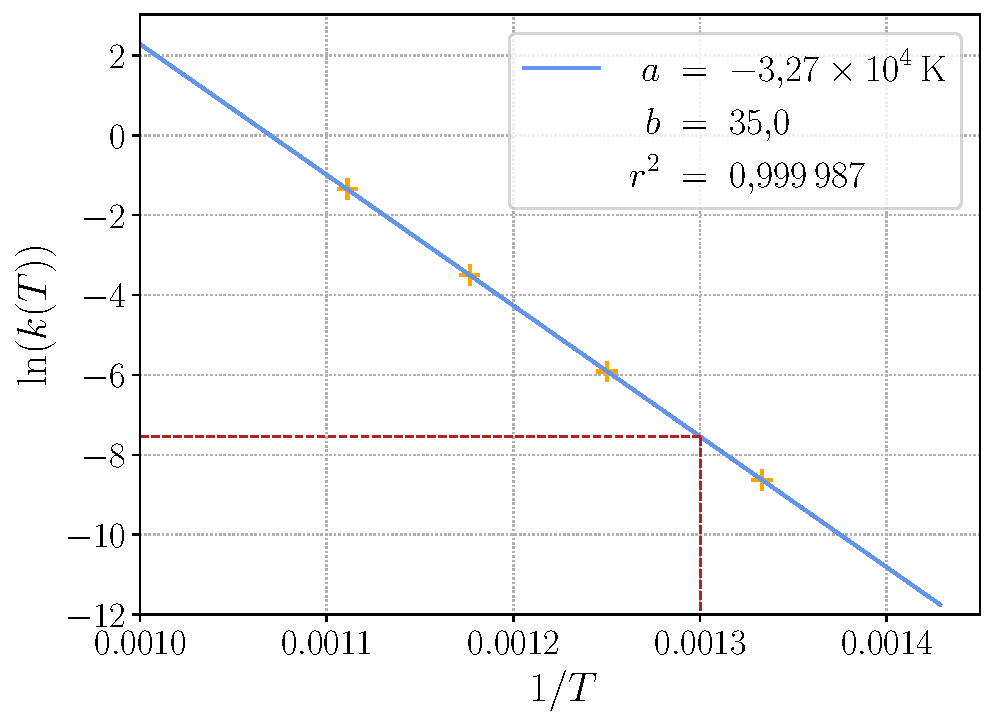
\includegraphics[width=\linewidth]{exo1_lnk}
		\end{center}
	\end{minipage}
}

\QR{%
	Quelle est la valeur de la constante de vitesse à
	\SI{500}{\degreeCelsius}~?
}{%
	Avec la régression linéaire précédente, on doit trouver la valeur de
	$\ln(k)$ avec $T = \SI{773}{K}$, c'est-à-dire $1/T =
		\SI{1.30e-3}{K^{-1}}$~: par lecture graphique, on trouve $\ln(k) =
		-\num{7.51}$, d'où
	\[\boxed{k(\SI{500}{\degreeCelsius}) = \SI{5.5e-4}{s^{-1}}}\]
}

\subsection{Utilisation du temps de demi-réaction}
\enonce{%
	Soit la réaction
	\[\ce{A -> B + C}\]
}
\QR{%
	Déterminer son ordre sachant que lorsqu'on multiplie par 10 la concentration
	initiale de A, on divise le temps de demi-réaction par 10.
}{%
	D'après le cours, pour une réaction d'ordre 2 en A uniquement, on a $t_{1/2} =
		\frac{1}{ka[\ce{A}]_0}$ avec $a$ le coefficient stœchiométrique du composé A.
	C'est la seule situation où augmenter la concentration baisse le temps de
	demi-réaction~: l'ordre 0 a un $t_{1/2} \propto [\ce{A}]_0$, et l'ordre 1 ne
	dépend pas de $[\ce{A}]_0$~: on a donc une \textbf{réaction d'ordre 2 en A}.
}
\end{document}
